\subsection{Coverage}
\label{sec::coverage}
The Dean feels that it is not economically justified to by a robot system for 595.176 DKK just to collect cups. Hence, it is interesting to have the robot do a second task, namely washing of the floors.\\[0.2cm]
All coverage is done online, and it involves the functions
\begin{itemize}\itemsep-2pt
\item \textbf{Online wavefront} from the robots current position to the center of an other room.
\item \textbf{Coverage of a room} is similar for every room.
\item \textbf{Collecting the cups} within a radius of 4px.
\item \textbf{Offline wavefront}, as described in section \ref{sec::planning}, when the robot has collected 20 cups and needs unload them at one of the unloading--stations, by using the 2D--array from the offline planning. 
\end{itemize}

\subsubsection{Solution}
The coverage plan for the complete map is
\begin{enumerate}\itemsep-2pt
\item Block A
\item The Big Hall
\item Block B
\item Block C
\item Block D
\item Block E
\end{enumerate}

Figure \ref{fig::room} illustrates covering a room. The dark gray pixels are where the robot is moving and the light gray area is what the robot has covered for cups. The coverage is done in the following steps
\begin{enumerate}\itemsep-2pt
\item Starts at upper left corner of the rooms freespace, $Q_{room}$, and keep moving down to the lower left corner of the $Q_{room}$.
\item Turn left 90 degrees and move 8 pixels
\item Turn left 90 degrees and keep moving until the limit of the $Q_{room}$ is detected.
\item Turn right 90 degrees and move 8 pixels
\item Turn right 90 degrees and keep moving until the limit of the $Q_{room}$ is detected.
\item Keep repeating the step 2 to 5 until the same y--coordinate as the upper right corner of the rooms $Q_{room}$ is detected. At this point, either the robot has the same position as the upper right corner or the lower right corner of the $Q_{room}$.    
\begin{itemize}\itemsep-2pt  
\item If it is position of the lower right corner of the $Q_{room}$, then turn 90 degrees to the left and keep moving until the robot has the same position as the upper right corner of the $Q_{room}$ (Case A on figure \ref{fig::room}). The room is fully covered and the robot can move to the next room. 
\item If it is position of the upper right corner of the $Q_{room}$, then turn right 90 degrees and keep moving until the robot has the same position as the lower right corner of the $Q_{room}$ (Case B on figure \ref{fig::room}). The room is fully covered and the robot can move to the next room. 
\end{itemize}
\end{enumerate} 
This coverage algorithm is very simple and it is only possible to use it, because all the rooms are squared. When the room is fully covered, then the center of the next room is popped from the priority queue of the block, that the robot is currently in. A wavefront is then generated from that center-position, until the wavefront hits the position of the robot, and then the path to that center is found. The wavefront is stopped as soon as it hits the robots position, because the robot will never gonna use the rest of wavefront, and it saves a lot of time and memory by not making a full wavefront map. This makes it also possible to run the wavefront online, because most often the robot does not have to drive so far to get to the next room center. 

\begin{figure}[H]
\centering
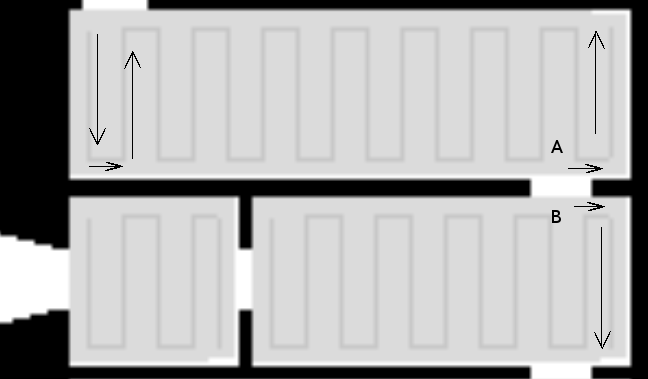
\includegraphics[scale=0.33]{img/room.png}
\caption{Coverage of a room in the complete map.}
\label{fig::room}
\end{figure}

Figure \ref{fig::coverage} shows the complete map covered with this projects program.

\begin{figure}[H]
\centering
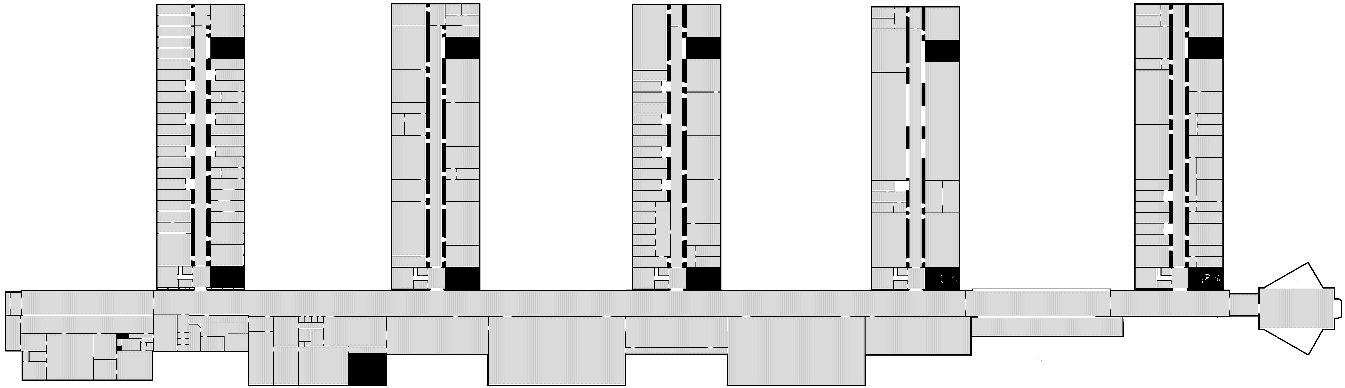
\includegraphics[scale=0.33]{img/coverage.png}
\caption{Coverage of the complete map.}
\label{fig::coverage}
\end{figure}

\subsubsection{Results of the planning and coverage}
The calculation of the path the robot takes is $time\:sec$.\\[0.2cm]
While the robot moves around in the map, a counter keeps track of how many pixels the robot had moved during that time. \\[0.2cm]
If only focusing on washing the floor, the robot moves $513.008\:px$. The time it takes it to clean the schools floor is then
$$t=\frac{513.008\:px}{50.000\:px/hour}=10,26\:hours$$
If the robot cleans the floor at night, e.g. from 8 PM to 6.15 AM, it would be realistic for it to do the job, without being interrupted or disturbed by the students. The program does not take into account for obstacles that suddenly appears, e.g. a university teacher, standing in one of the classrooms, writing something on a blackboard. Also, it would not be pleasant for the teacher to be hit by the robot, with a speed of 5 km/hour.\\[0.2cm]

Assuming that 
\begin{itemize}\itemsep-2pt
\item One man hour cost 208 DKK 
\item The cleaning lady works within the normal working hours 
\item She uses a washing machine with the same speed and and radius, as the robot
\item She uses a normal workday (8 hours) on cleaning the same area.
\item The robot does not need maintenance.
\end{itemize}  
then, it still would be feasible for the dean to invest in this robot. In the long run, a cleaning of the floor, done by the cleaning lady, would cost the dean 1664 DKK. If the floor needs to be cleaned every 24 hours, then at one point, within the robots durability, it will make a profit. Saying a cleaning robot costs 595.176 DKK, then approximately after a year it will by paid of, by the saved man hours used on cleaning the floor. 